%--------- CHAPITRE 2 ---------
\chapter{LoRaWAN et LR-FHSS}
\label{chap2}

\section{Introduction}
Ce chapitre présente en détail les spécifications techniques du \gls{lrfhss} et les points de divergence avec LoRa. Ces spécifications constituent le socle technique sur lequel repose notre travail d'optimisation. Nous verrons comment cette nouvelle approche, en rupture avec le LoRa, ouvre la voie à des réseaux IoT massifs déployés, tant sur Terre que dans l'espace.

\section{Évolution de LoRa vers LR-FHSS}
LoRa, acronyme de \textit{Long Range}, est une technologie \textit{\gls{lpwan}} qui a révolutionné le monde de l'\gls{iot} depuis son apparition. Conçue pour permettre des communications longue portée à faible consommation énergétique, elle a rapidement suscité l'intérêt tant des chercheurs que des industriels, donnant lieu à une multitude d'applications allant de la surveillance environnementale à la gestion intelligente des villes.

Cependant, face à l'explosion du nombre de capteurs connectés et aux besoins croissants en capacité réseau, les limitations du LoRa sont devenues manifestes, particulièrement dans les environnements urbains denses. C'est dans ce contexte que la technologie \gls{lrfhss} a émergé, apportant une réponse innovante à ces défis de scalabilité.

\subsection{Limites du LoRa}
Le LoRa repose sur une modulation CSS (\textit{Chirp Spread Spectrum}) qui offre d'excellentes performances en termes de portée et de consommation énergétique. Toutefois, cette approche présente des limitations dans les scénarios de déploiement massif. Lorsque plusieurs dispositifs tentent de communiquer dans la même zone géographique, les collisions de paquets deviennent nombreuses et inévitables, conduisant à une dégradation significative des performances réseau.

Ces limitations ont été largement documentées dans la littérature scientifique, motivant la recherche de solutions capables de supporter des milliers de nœuds dans les réseaux IoT \cite{free}. C'est précisément pour répondre à ces défis que Semtech a développé le \gls{lrfhss}.

\subsection{Origines et objectifs du LR-FHSS}

Introduit par Semtech et standardisé par la LoRa Alliance en 2020 \cite{loraalliance2020regional}, le \gls{lrfhss} a un double objectif pour répondre à l'évolution des besoins actuels :

\begin{itemize}
	\item \textbf{Augmenter considérablement la capacité des réseaux terrestres} : En environnement urbain dense, où le spectre radio est une ressource très convoitée, le LR-FHSS propose une meilleure utilisation de cette ressource.
	
	\item \textbf{Étendre LoRaWAN aux communications satellitaires directes} : L'émergence des constellations de satellites en orbite basse (\gls{leo}) offre une opportunité de connecter des capteurs situés dans des zones blanches non couvertes par les réseaux terrestres traditionnels. Le \gls{lrfhss}, avec sa robustesse aux perturbations et sa capacité à fragmenter les données, se montre particulièrement adapté à ce contexte exigeant \cite{ieee_lr_fhss_2021, lr_fhss_dts}.
\end{itemize}

\subsection{Différence entre LoRa et LR-FHSS} 

Le \gls{lrfhss} marque une rupture fondamentale avec le \gls{lora}. Là où le LoRa ajuste la robustesse de la liaison par variation du facteur d'étalement (\gls{sf}), le LR-FHSS adopte une approche totalement différente :

\begin{enumerate}
	\item \textbf{Abandon du \textit{\gls{css}}} : La modulation \gls{gmsk} remplace les chirps et offre une occupation spectrale plus compacte et mieux maîtrisée.
	
	\item \textbf{Étalement par saut de fréquence intra-paquet} : Plutôt que d'étaler le signal dans le temps sur une large bande fixe, le LR-FHSS fragmente le message en petits morceaux transmis sur des sous-canaux très étroits (488 Hz), en changeant dynamiquement de fréquence au sein même d'un paquet.
\end{enumerate}

Cette approche, inspirée des techniques militaires de résistance au brouillage et à l'écoute, permet une utilisation optimale du spectre disponible tout en offrant une forte résistance face aux interférences \cite{semtech2022lrfhss}.

\section{Architecture physique du LR-FHSS}

L’architecture physique du LR-FHSS repose sur un ensemble de mécanismes visant à optimiser l’utilisation du spectre radio et à améliorer la robustesse des transmissions. Dans cette section, nous présentons d’abord le principe de découpage spectral, avant d’examiner les différentes configurations de débits de données définies par la spécification.

\subsection{Principe de découpage spectral}

L'innovation majeure du \gls{lrfhss} réside dans sa manière de découper finement le spectre radio. Contrairement au LoRa, qui utilise des canaux de 125 kHz, le LR-FHSS divise une large bande appelée \textit{Operating Channel Width} (OCW) en une multitude de sous-canaux de seulement 488 Hz chacun. Cette granularité spectrale est la clé de la capacité élevée de cette modulation.

En pratique, chaque fragment de données occupe une bande passante instantanée (\textit{Occupied Bandwidth} - OBW) de 488 Hz, et la transmission d'un paquet complet implique de sauter d'un sous-canal à un autre selon un schéma pseudo-aléatoire. Cette solution technique présente plusieurs avantages :

\begin{itemize}
	\item \textbf{Diversité fréquentielle} : En répartissant un même message sur différentes fréquences, on réduit la probabilité qu'une interférence à bande étroite détruise l'intégralité du paquet.
	
	\item \textbf{Réduction des collisions} : Même si deux dispositifs transmettent simultanément, la probabilité qu'ils utilisent exactement les mêmes sous-canaux au même moment devient faible.
	
	\item \textbf{Utilisation équitable du spectre} : Le saut aléatoire garantit une distribution statistiquement uniforme de l'occupation spectrale.
\end{itemize}

\subsection{Configurations des débits de données (DR)}

La spécification de la LoRa Alliance \cite{loraalliance2025regional} définit quatre configurations principales pour le LR-FHSS, désignées par les débit de données (\textit{Data Rates}- DR) DR8 à DR11 pour la zone européenne. Ces configurations diffèrent par la largeur de la bande de canal (OCW) et le taux de codage (Coding Rate - CR) appliqué.

Le tableau suivant présente ces configurations pour la région européenne (\gls{etsi}) :

\begin{table}[H]
	\centering
	\caption{Configuration des débits de données LR-FHSS (DR8--DR11)}
	\resizebox{\textwidth}{!}{%
		\begin{tabular}{|c|c|c|c|c|}
			\hline
			Débit de données (DR)& Bande de saut (OCW) & Taux de codage (CR) & Nombre de canaux & Débit physique (bps) \\
			\hline
			DR8  & 137 kHz & 1/3 & 280 & 162 \\
			DR9  & 137 kHz & 2/3 & 280 & 325 \\
			DR10 & 336 kHz & 1/3 & 688 & 162 \\
			DR11 & 336 kHz & 2/3 & 688 & 325 \\
			\hline
		\end{tabular}%
	}
\end{table}
Ces configurations de DR ont certaines particularités :

\begin{itemize}
	\item \textbf{Compromis entre robustesse et débit} : Les configurations avec CR 1/3 (DR8 et DR10) privilégient la robustesse au détriment du débit physique, idéales pour maximiser la portée ou la fiabilité dans des conditions difficiles. À l'inverse, les configurations CR 2/3 (DR9 et DR11) doublent le débit physique, mais avec moins de protection contre les erreurs.
	
	\item \textbf{Nombre de canaux disponibles} : Plus l'OCW est large, plus le nombre de canaux physiques disponibles est élevé. Ainsi, DR10 et DR11 offrent 688 canaux physiques, contre  280 pour DR8 et DR9. Cette abondance de canaux est fondamentale pour supporter un grand nombre de dispositifs simultanés.
	
	\item \textbf{Variations régionales} : D'autres régions, comme la FCC (Federal Communications Commission - Amérique du Nord), bénéficient d'allocations spectrales différentes avec des OCW pouvant atteindre 1,523 MHz et une grille de 25,4 kHz, offrant ainsi environ 60 canaux utilisables, soit une capacité encore supérieure.
\end{itemize}

\section{Structure du paquet LR-FHSS}

Cette section présente d’abord l’anatomie d’une trame physique, puis décrit les
différents composants constituant un paquet LR-FHSS ainsi que le mécanisme de saut de fréquence associé.

\subsection{Anatomie d'une trame physique}

La structure d'un paquet LR-FHSS a été conçue avec un objectif principal : assurer une robustesse maximale de la transmission. Pour y parvenir, les concepteurs ont opté pour une redondance intelligente de l'en-tête, élément critique contenant les informations nécessaires à la démodulation du reste du paquet. Le reste de la charge utile est fragmenté en blocs de longueur fixe.
Le tableau suivant détaille cette structure :

\begin{table}[htbp]
	\centering
	\caption{Structure détaillée d'un paquet LR-FHSS}
	\label{tab:packet_structure}
	\small
	\begin{tabular}{|p{3cm}|p{7cm}|p{5cm}|}
		\hline
		\textbf{Élément} & \textbf{Composants} & \textbf{Spécifications} \\
		\hline
		\textbf{En-tête (PHDR)} & 
		\parbox[t]{7cm}{
			\begin{itemize}[leftmargin=*,nosep]
				\item Préambule (114 échantillons)
				\item Mot de synchronisation (0x2C0F7995)
				\item PHDR (4 octets)
				\item CRC de l'en-tête (1 octet)
		\end{itemize}} & 
		\parbox[t]{4cm}{
			Répété $N$ fois: 
			\begin{itemize}[leftmargin=*,nosep]
				\item $N=3$ si CR 1/3
				\item $N=2$ si CR 2/3
				\item Durée : 233,472 ms
		\end{itemize}} \\
		\hline
		\textbf{Charge utile} & 
		\parbox[t]{8cm}{
			\begin{itemize}[leftmargin=*,nosep]
				\item Données PHY ($L$ octets)
				\item CRC de la charge utile (2 octets)
		\end{itemize}} & 
		\parbox[t]{5cm}{
			\begin{itemize}[leftmargin=*,nosep]
				\item Codage convolutionnel appliqué
				\item Dure 102,4 ms
				\item Sauts de fréquence entre fragments
		\end{itemize}} \\
		\hline
	\end{tabular}
\end{table}

\subsection{Mécanisme de saut de fréquence}

Le cœur du LR-FHSS repose sur un mécanisme de saut de fréquence intra-paquet. Contrairement aux implémentations FHS traditionnelles où le signal est transmis séquentiellement sur une fréquence donnée pendant un temps défini, le LR-FHSS fragmente le paquet en blocs indépendants transmis sur différentes sous-porteuses. Cette dispersion fréquentielle intra-paquet améliore la robustesse aux collisions et aux interférences dans les réseaux denses.

\subsubsection{Principe de fonctionnement}

Le processus de saut suit une logique bien définie, illustrée par la spécification RP002-1.0.5 \cite{loraalliance2025regional} :

\begin{enumerate}
	\item \textbf{Sélection aléatoire du point de départ} : Avant de commencer la transmission, l'émetteur choisit aléatoirement une fréquence initiale parmi l'ensemble des sous-canaux disponibles. Cette initialisation aléatoire garantit une distribution statistique uniforme de l'occupation spectrale à l'échelle du réseau.
	
	\item \textbf{Annonce du pattern de saut} : Le \textit{\gls{phdr}} contient un identifiant du pattern de saut qui sera utilisé pour le reste du paquet. Cet identifiant permet au récepteur de savoir sur quelles fréquences chercher les fragments suivants.
	
	\item \textbf{Exécution du saut} : Au cours de la transmission, l'émetteur saute de fréquence selon le pattern annoncé. La séquence de saut est pseudo-aléatoire mais déterministe : connaissant l'identifiant du pattern et la fréquence initiale, le récepteur suit la communication.
\end{enumerate}

\subsubsection{Périodicité du saut}

La périodicité du changement de fréquence n'est pas uniforme sur toute la durée du paquet. Elle diffère entre l'en-tête et la charge utile :

\begin{itemize}
	\item \textbf{En-tête (PHDR)} : Chaque répétition de l'en-tête dure \textbf{233,472 ms} et est transmise sur une fréquence différente. Ainsi, avec $N=3$ répétitions (CR 1/3), l'en-tête occupe environ 700 ms au total, réparti sur trois sous-canaux distincts.
	
	\item \textbf{Charge utile} : Chaque fragment de la charge utile dure \textbf{102,4 ms} et occupe un nouveau sous-canal. Pour un message de quelques dizaines d'octets, cela représente plusieurs dizaines de sauts de fréquence, répartissant ainsi la charge utile sur une large portion du spectre disponible.
\end{itemize}

Cette différence de périodicité s'explique par les contraintes respectives de chaque partie du paquet. L'en-tête doit être détectable rapidement et de manière fiable, justifiant des segments plus longs. La charge utile, en revanche, bénéficie d'une granularité temporelle plus fine pour maximiser la diversité fréquentielle.

\begin{figure}[htbp]
	\centering
	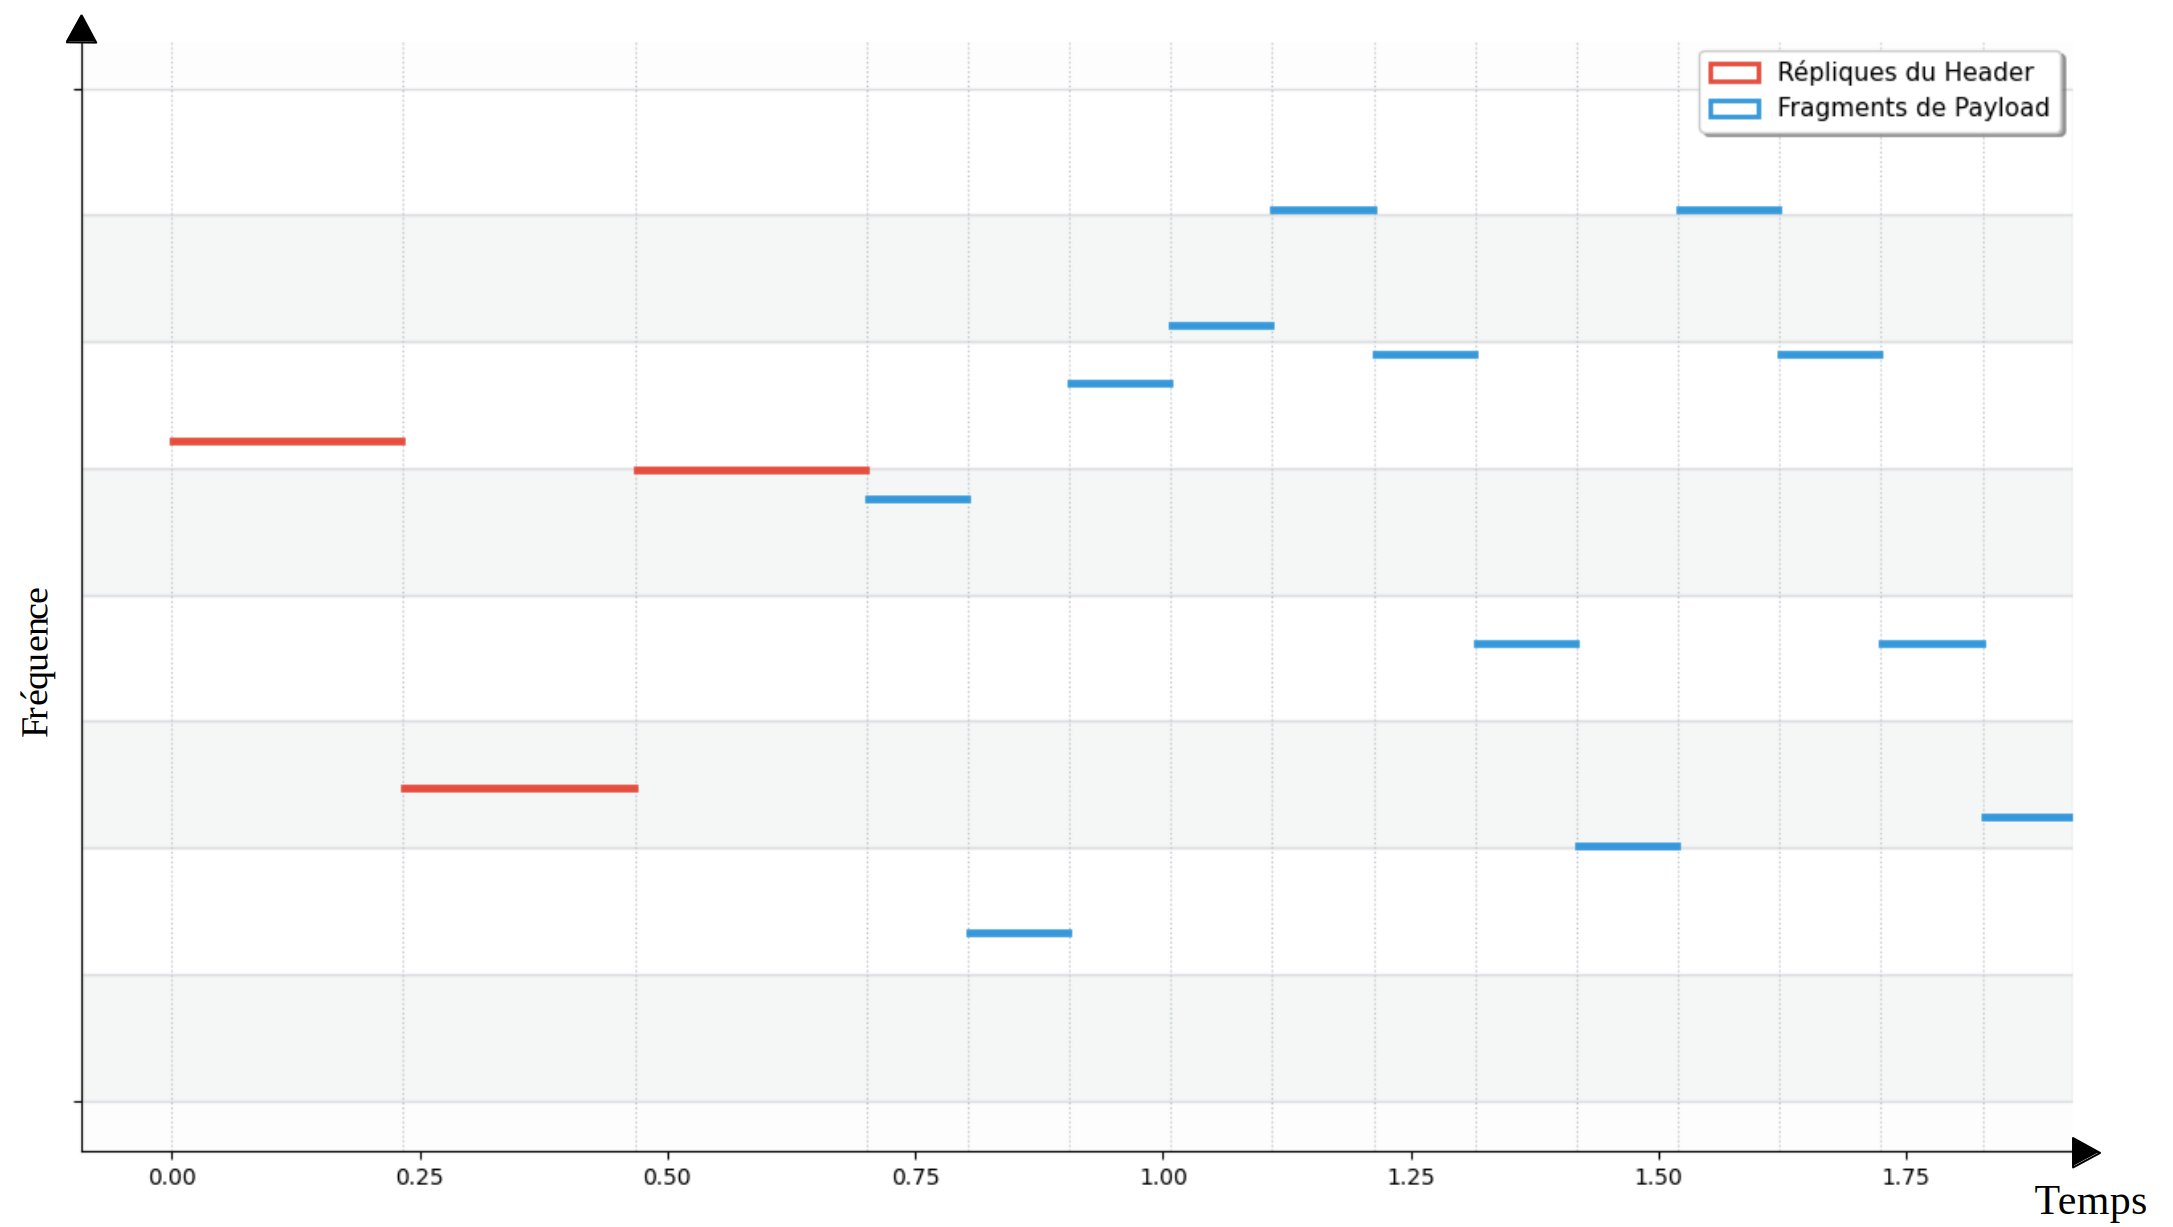
\includegraphics[width=1\textwidth]{images/lr_fhss_hop.png}
	\caption{Illustration des sauts de fréquence LR-FHSS}
	\label{fig:lr_fhss_hop}
\end{figure}

\section{Calcul du temps d'antenne}
Le temps d’antenne (Time on Air – ToA) constitue un paramètre essentiel dans l’analyse des performances des transmissions LR-FHSS. Cette section présente d’abord l’importance du temps d’antenne dans les réseaux IoT, puis introduit la formule générale permettant de le calculer avant de détailler le calcul du temps associé à la charge utile.

\subsection{Importance du temps d'antenne}

Dans les réseaux IoT, le temps d'antenne ($ToA$) est une métrique critique pour deux raisons principales :

\begin{itemize}
	\item \textbf{Respect de la réglementation} : Les bandes ISM (Industrial, Scientific and Medical) utilisées par LoRaWAN sont soumises à des contraintes de \textit{duty cycle}, limitant le pourcentage de temps pendant lequel un dispositif peut émettre (typiquement 1\% en Europe). Un $ToA$ élevé réduit donc la fréquence à laquelle un capteur peut transmettre.
	
	\item \textbf{Consommation énergétique} : La radio étant le composant le plus énergivore d'un capteur IoT, minimiser le $ToA$ est essentiel pour prolonger la durée de vie de la batterie.
\end{itemize}
\subsection{Formule générale}

Le temps d'antenne total d'un paquet LR-FHSS se décompose en deux parties : le temps de transmission de l'en-tête et le temps de transmission de la charge utile. La formule générale s'écrit :

\[ ToA = T_{header} + T_{payload} \]

où :

\[ T_{header} = N \times 233{,}472\,\text{ms} \]

avec $N$ le nombre de répétitions de l'en-tête ($N=3$ pour CR 1/3, $N=2$ pour CR 2/3).

\subsection{Calcul du temps de la charge utile}

Le calcul du temps de la charge utile, $T_{\text{payload}}$ est plus complexe, car il dépend de la longueur du message, du taux de codage et de la structure de fragmentation. Les formules suivantes sont extraites de la spécification RP002-1.0.5 \cite{loraalliance2025regional} :

\begin{itemize}
	\item \textbf{Pour CR = 1/3} :
	\begin{equation}
		\label{eq:toa1}
		 T_{payload} = \frac{(8 \times (L + 2) + 6) \times 3 + \left\lceil \frac{(8 \times (L + 2) + 6) \times 3}{48} \right\rceil \times 2}{50} \times 102{,}4\,\text{ms}
	\end{equation}
	
	
	\item \textbf{Pour CR = 2/3 (débit élevé)} :
	\begin{equation}
		\label{eq:toa2}
		 T_{payload} = \frac{\frac{(8 \times (L + 2) + 6) \times 3}{2} + \left\lceil \frac{(8 	\times (L + 2) + 6) \times 3}{2 \times 48} \right\rceil \times 2}{50} \times 102{,}4\,\text{ms} 
	\end{equation}
	
\end{itemize}

où $L$ est la longueur du message en octets (sans compter le CRC de 2 octets ajouté automatiquement).

Ces formules reflètent les opérations successives appliquées aux données :

\begin{enumerate}
	\item \textbf{$(8 \times (L + 2) + 6)$} : Calcul du nombre total de bits à transmettre, incluant le message ($L$ octets), le CRC (2 octets) et quelques bits supplémentaires de bourrage.
	
	\item \textbf{Multiplication par 3 ou par 3/2} : Application du codage convolutionnel qui ajoute de la redondance. Un taux 1/3 signifie que chaque bit d'information génère 3 bits codés.
	
	\item \textbf{Division par 48 et arrondi supérieur} : Découpage en blocs de 48 bits codés (un fragment), avec ajout d'un fragment supplémentaire si nécessaire.
	
	\item \textbf{Multiplication par 102,4 ms} : Durée d'un fragment.
\end{enumerate}

\section{Performances et capacité du LR-FHSS}
Cette section présente les performances et la capacité du LR-FHSS. Elle examine d’abord les apports théoriques issus de la littérature, puis détaille les validations expérimentales dans différents contextes, y compris les scénarios satellitaires, et enfin discute de l’efficacité énergétique du système.

\subsection{Apports théoriques}

L'architecture du LR-FHSS offre des avantages majeurs par rapport au LoRa. Plusieurs études académiques ont démontré ses bénéfices théoriques :

\subsubsection{Capacité réseau décuplée}

Dans cette étude \cite{lr_fhss_overview}, les auteurs ont réalisé une analyse comparative détaillée entre LoRa CSS et LR-FHSS. Leurs travaux montrent que, grâce à la granularité spectrale fine (488 Hz par fragment contre 125 kHz pour un canal LoRa classique), le LR-FHSS peut théoriquement supporter jusqu'à dix fois plus de dispositifs dans un même environnement. Cette multiplication de la capacité s'explique par deux phénomènes :

\begin{itemize}
	\item \textbf{Réduction des collisions} : La probabilité que deux dispositifs utilisent exactement les mêmes sous-canaux au même instant est considérablement réduite. Même en cas de collision partielle (quelques fragments communs), les fragments non corrompus peuvent parfois suffire à reconstruire le message grâce au codage convolutionnel.
	
	\item \textbf{Utilisation optimale du spectre} : Le saut aléatoire généré par l'algorithme \textit{Linear Feedback Shift Register (LFSR)} \cite{lfsr} garantit une distribution uniforme de la charge sur l'ensemble du spectre disponible.
\end{itemize}

Dans l'étude \cite{arxiv_lrfhss_2020}, les auteurs ont confirmé ces résultats par des modélisations analytiques, établissant des bornes théoriques sur le nombre maximal de dispositifs supportés en fonction du taux de charge offert et de la configuration choisie (DR, CR).

\subsubsection{Robustesse aux interférences}

La fragmentation et la dispersion fréquentielle confèrent au LR-FHSS une robustesse exceptionnelle face aux interférences, qu'elles soient d'origine naturelle (bruit impulsif, affaiblissement sélectif en fréquence) ou anthropique (brouilleurs, autres systèmes radio).

Semtech, dans sa note d'application AN1200.64 \cite{semtech2022lrfhss}, montre que le LR-FHSS maintient un taux de réception élevé même en présence d'interférences sur les bandes étroites qui bloqueraient complètement un canal LoRa. Cette résilience s'explique par le fait qu'une interférence localisée en fréquence ne détruit qu'une partie des fragments LR-FHSS, le reste restant exploitable.

\subsection{Validation expérimentale}

Cette section analyse les performances et la capacité de cette modulation à travers trois aspects principaux : les apports théoriques mis en évidence dans la littérature, les validations expérimentales réalisées dans différents scénarios, ainsi que l’efficacité énergétique du système.

\subsubsection{Analyses réelles}

La validation expérimentale est cruciale pour confirmer les performances réelles du LR-FHSS. À cet égard, les auteurs de l'étude \cite{lr_fhss_traces} ont mené une analyse approfondie sur des traces de paquets capturées en conditions réelles auprès de réseaux opérationnels. Leurs résultats confirment l'utilisation équitable du spectre, les mesures démontrant que tous les sous-canaux sont sollicités de manière équiprobable grâce au saut de fréquence aléatoire. 

Par ailleurs, l'étude révèle que les collisions partielles, limitées à quelques fragments, sont nettement plus fréquentes que les collisions totales ; grâce à la robustesse du codage, la majorité de ces interférences ne compromettent pas la récupération du message. Enfin, les auteurs soulignent une sensibilité marquée des performances vis-à-vis du choix des débits de données (DR) et du taux de codage (CR).

Une autre contribution majeure à la validation expérimentale a été apportée par cette étude \cite{lrfhss_comparaison}, où les auteurs ont réalisé une campagne de mesures comparative entre le LR-FHSS et le LoRa. L'étude montre que, dans des scénarios de non-ligne de vue (NLoS), le LR-FHSS (particulièrement aux DR8 et DR10) maintient une connectivité fiable jusqu'à 4 km, là où le LoRa (même au SF12) subit une perte totale de signal dès 2 km.

\subsubsection{Scénarios satellitaires}

L'un des cas d'usage les plus prometteurs du LR-FHSS concerne les communications directes avec des satellites en orbite basse terrestre. Ce scénario, extrêmement exigeant en raison de l'effet Doppler (décalage de fréquence), de l'atténuation de l'espace libre et des contraintes de puissance d'émission, constitue un cadre d'essai idéal pour évaluer la robustesse du LR-FHSS.

Dans l'étude \cite{lepcha_application_2021}, il est clairement démontré que l'utilisation de satellites en orbite basse pour la collecte de données dans des zones reculées et à faible coût avec LoRaWAN est faisable. Cela confirme naturellement les performances attendues du LR-FHSS, conçu d'une part pour répondre à ce besoin spécifique.

Les auteurs dans \cite{ieee_lr_fhss_2021} ont simulé des liaisons montantes LoRaWAN vers des satellites LEO en intégrant les effets physiques réels (Doppler, bruit thermique, fenêtre de visibilité). Leurs résultats démontrent que le LR-FHSS, en particulier avec CR 1/3, peut maintenir un lien fiable même dans ces conditions hostiles, là où le LoRa CSS peine à assurer la connectivité.

Dans cette étude \cite{lr_fhss_dts}, les auteurs ont approfondi cette analyse en comparant différentes configurations de LR-FHSS et en évaluant l'impact de paramètres orbitaux (altitude, inclinaison) sur les performances. Ils concluent que le LR-FHSS représente une solution viable pour l'IoT spatial, à condition d'optimiser la sélection des paramètres en fonction des contraintes.

Plus récemment, dans ce travail \cite{doppler_limits}, les auteurs ont étudié les limites fondamentales imposées par l'effet Doppler sur le LR-FHSS dans un contexte satellitaire. Ils montrent que, moyennant des techniques de pré-compensation ou de correction adaptative, le LR-FHSS peut fonctionner sur des liaisons satellitaires avec des vitesses relatives de plusieurs km/s, ouvrant ainsi la voie à des constellations massives de satellites à basse altitude pour l'IoT global.

\subsection{Efficacité énergétique}

À première vue, le LR-FHSS semble moins avantageux que le LoRa CSS en raison d’un temps d’antenne (ToA) plus long, augmentant ainsi la consommation d’énergie par paquet. Ce constat est d'autant plus vrai au-delà de +14 dBm, seuil à partir duquel l’amplificateur haute puissance (HPA) provoque une hausse marquée du courant \cite{ullah2024_energy}. Toutefois, cette analyse isolée du temps de transmission n'est pas représentative. Grâce à sa forte robustesse face aux interférences et à l’effet Doppler, le LR-FHSS limite considérablement les retransmissions. 

En tenant compte de la probabilité réelle de succès, le LR-FHSS en DR9 peut ainsi consommer moins d’énergie par paquet transmis que le LoRa DR5 sur des liaisons longue distance, selon \cite{SanchezVital2024EnergyLRFHSS, ullah2024_energy}. Dans des conditions optimales (DR9 ou DR11, mode non acquitté, charge utile maximale), il est même possible d’atteindre une autonomie théorique de 16 ans avec une simple pile bouton pour une transmission quotidienne \cite{SanchezVital2024EnergyLRFHSS}. L’efficacité énergétique du LR-FHSS ne peut donc pas être évaluée uniquement à partir du $ToA$, mais doit être appréciée de manière globale, en intégrant la fiabilité du lien, la taille des données transmises et la périodicité des envois.

\section{Conclusion}

Ce chapitre a présenté en détail les spécifications techniques du protocole LR-FHSS. Nous avons exploré les principes fondamentaux de cette technologie, depuis son architecture physique basée sur le saut de fréquence intra-paquet jusqu'à ses performances validées expérimentalement.

La compréhension approfondie des mécanismes du LR-FHSS, acquise dans ce chapitre, constitue le socle indispensable pour concevoir et évaluer des solutions d'optimisation. Les spécifications techniques présentées ici serviront de référence tout au long de ce mémoire, guidant nos choix de modélisation et de validation expérimentale.